
\chapter{THIẾT KẾ GIẢI PHÁP VÀ QUY TRÌNH HỌC MÁY}

% ============================================
% 2.1. TỔNG QUAN GIẢI PHÁP
% ============================================

\section{Tổng quan giải pháp và quy trình học máy}

\subsection{Định hướng xây dựng giải pháp}

Đề tài ``Phân loại cảm xúc từ phản hồi của sinh viên'' được xây dựng theo hướng học máy có giám sát, sử dụng dữ liệu văn bản đã được gán nhãn để huấn luyện và đánh giá mô hình phân loại.

Mục tiêu của giải pháp là chuyển đổi các phản hồi dưới dạng ngôn ngữ tự nhiên thành biểu diễn số, từ đó áp dụng các thuật toán học máy để dự đoán nhãn cảm xúc tương ứng.

Trong phạm vi học phần Nhập môn Học máy, nhóm lựa chọn hai phương pháp biểu diễn văn bản là Bag-of-Words (BoW) và Term Frequency--Inverse Document Frequency (TF-IDF), kết hợp với hai thuật toán phân loại Multinomial Naive Bayes và K-Nearest Neighbors (K-NN).

Các phương pháp này phù hợp với phạm vi kiến thức của học phần, cho phép xây dựng quy trình xử lý tương đối rõ ràng và thực hiện các thí nghiệm so sánh có hệ thống.

Nhóm sử dụng ngôn ngữ Python cùng các thư viện Pandas, NumPy, Scikit-learn và SciPy để triển khai quy trình học máy.

Giải pháp được tổ chức thành các giai đoạn chính: khám phá dữ liệu, tiền xử lý, phân chia dữ liệu, biểu diễn đặc trưng, huấn luyện, lựa chọn tham số, đánh giá và phân tích lỗi.


\subsection{Sơ đồ quy trình học máy}

Quy trình tổng thể được xây dựng dựa trên hướng dẫn của học phần, từ dữ liệu thô đến kết quả đánh giá cuối cùng.

Sơ đồ~\ref{sd:quy-trinh-hoc-may} trình bày các bước thực hiện trong đề tài.

\begin{sodo}[H]
    \centering

    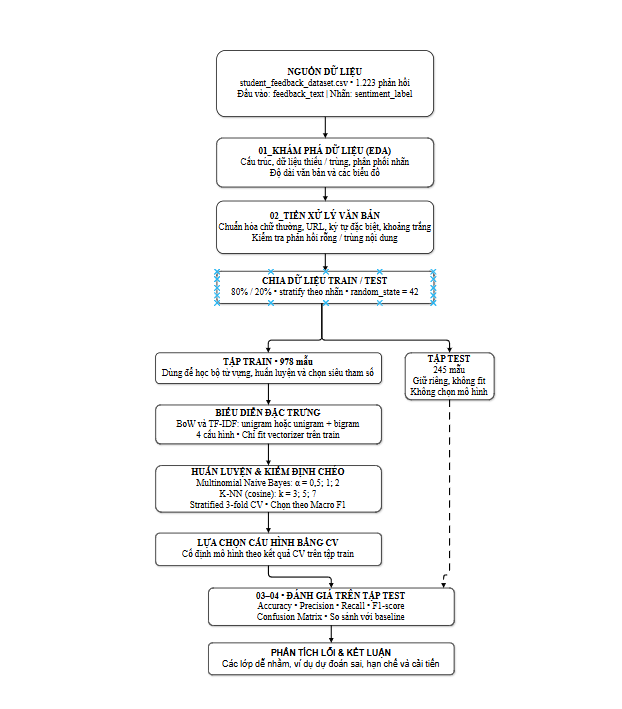
\includegraphics[
        width=0.98\textwidth,
        height=0.78\textheight,
        keepaspectratio
    ]{images/so_do_quy_trinh_hoc_may.png}

    \caption{Quy trình học máy áp dụng cho đề tài}
    \label{sd:quy-trinh-hoc-may}
\end{sodo}

Quy trình được thực hiện theo thứ tự nhằm bảo đảm tính nhất quán giữa các giai đoạn.

Trong đó, tập dữ liệu kiểm thử được tách riêng trước khi xây dựng bộ từ vựng và huấn luyện mô hình. Việc lựa chọn siêu tham số được thực hiện trên tập huấn luyện thông qua kiểm định chéo, không sử dụng kết quả tập kiểm thử để lựa chọn mô hình.

Điều này giúp hạn chế hiện tượng rò rỉ dữ liệu (Data Leakage) và hỗ trợ đánh giá khả năng khái quát hóa của mô hình.


% ============================================
% 2.2. TIỀN XỬ LÝ VĂN BẢN
% ============================================

\section{Tiền xử lý dữ liệu văn bản}

\subsection{Mục đích tiền xử lý}

Dữ liệu phản hồi ban đầu được lưu dưới dạng văn bản tự nhiên. Văn bản có thể chứa chữ hoa, chữ thường, dấu câu, khoảng trắng thừa và một số thành phần không cần thiết cho quá trình biểu diễn đặc trưng.

Tiền xử lý văn bản nhằm tạo ra một định dạng thống nhất, giúp các phương pháp vector hóa xử lý dữ liệu hiệu quả và hạn chế những khác biệt không cần thiết giữa các cách viết.

Tuy nhiên, đối với bài toán phân loại cảm xúc, một số thành phần văn bản có thể chứa thông tin hữu ích. Vì vậy, nhóm lựa chọn phương pháp làm sạch tương đối đơn giản, tránh loại bỏ từ ngữ một cách máy móc.

Quá trình tiền xử lý được thực hiện trong notebook \texttt{02\_Preprocessing.ipynb}, sử dụng hàm \texttt{clean\_text()} được xây dựng trong module \texttt{src/text\_utils.py}.


\subsection{Các bước làm sạch văn bản}

Quy trình làm sạch văn bản của nhóm gồm các bước chính:

\begin{enumerate}
    \item \textbf{Chuẩn hóa chữ thường:}

    Chuyển toàn bộ nội dung văn bản về dạng chữ thường nhằm giảm sự khác biệt giữa những từ có cùng nội dung nhưng khác cách viết hoa.

    \item \textbf{Xử lý đường dẫn URL:}

    Những chuỗi có dạng liên kết HTTP, HTTPS hoặc bắt đầu bằng \texttt{www} được thay thế bằng khoảng trắng.

    \item \textbf{Xử lý dấu câu và ký tự đặc biệt:}

    Loại bỏ những dấu câu và ký tự không cần thiết theo quy tắc làm sạch đã xây dựng. Nhóm giữ lại chữ cái Unicode, chữ số, khoảng trắng và dấu nháy đơn.

    \item \textbf{Chuẩn hóa khoảng trắng:}

    Các khoảng trắng liên tiếp được thay thế bằng một khoảng trắng duy nhất. Đồng thời loại bỏ khoảng trắng ở đầu và cuối chuỗi.

    \item \textbf{Giữ lại những từ có khả năng mang thông tin cảm xúc:}

    Nhóm không chủ động loại bỏ stopword, chữ số hoặc những từ phủ định như \texttt{not}, \texttt{no} và \texttt{never}.
\end{enumerate}

Việc giữ các từ phủ định là một quyết định quan trọng, bởi chúng có thể làm thay đổi ý nghĩa của câu.

Chẳng hạn, hai cụm từ ``good'' và ``not good'' có sắc thái khác nhau. Nếu loại bỏ từ ``not'', mô hình có thể mất một phần thông tin liên quan đến cảm xúc của văn bản.

Ngoài ra, nhóm không thực hiện stemming hoặc lemmatization trong quy trình hiện tại nhằm giữ phạm vi tiền xử lý đơn giản và thống nhất giữa các thí nghiệm.

Cần lưu ý rằng việc loại bỏ dấu câu hoặc URL vẫn có thể làm mất một số thông tin ngữ nghĩa. Đây là một hạn chế của quy trình tiền xử lý được nhóm xem xét khi phân tích kết quả.


\subsection{Kiểm tra dữ liệu không hợp lệ và trùng lặp}

Sau khi làm sạch văn bản, nhóm tiến hành kiểm tra các bản ghi trước khi chia dữ liệu.

Những trường hợp được xem xét bao gồm:

\begin{itemize}
    \item Phản hồi có nội dung rỗng sau khi làm sạch.

    \item Bản ghi bị thiếu nhãn mục tiêu.

    \item Các phản hồi có nội dung giống nhau nhưng được gán nhiều nhãn khác nhau.

    \item Các phản hồi có nội dung trùng lặp.
\end{itemize}

Đối với những nội dung giống nhau nhưng có nhãn mâu thuẫn, quy trình được thiết kế để loại bỏ nhóm bản ghi liên quan và lưu lại thông tin nhằm phục vụ kiểm tra.

Những nội dung trùng lặp còn lại được loại bỏ trước khi chia Train/Test, nhằm hạn chế khả năng một phản hồi giống nhau xuất hiện đồng thời trong cả hai tập dữ liệu.

Trên bộ dữ liệu thực tế đang sử dụng, các bước kiểm tra không phát hiện bản ghi cần loại bỏ do thiếu thông tin, trùng nội dung hoặc nhãn mâu thuẫn.

Vì vậy, số lượng dữ liệu sau bước kiểm tra vẫn là 1.223 phản hồi.

Nhóm sử dụng cột \texttt{feedback\_text} để tạo văn bản đầu vào và cột \texttt{sentiment\_label} làm nhãn mục tiêu. Những thuộc tính như \texttt{emotion\_tag} và \texttt{preprocessed\_text} không được đưa vào mô hình như các đặc trưng bổ sung, nhằm giữ đúng phạm vi phân loại dựa trên nội dung phản hồi gốc.


% ============================================
% 2.3. PHÂN CHIA DỮ LIỆU
% ============================================

\section{Phân chia dữ liệu huấn luyện và kiểm thử}

\subsection{Phương pháp chia dữ liệu}

Sau khi hoàn thành bước kiểm tra và làm sạch, nhóm sử dụng hàm \texttt{train\_test\_split()} của thư viện Scikit-learn để phân chia dữ liệu.

Tỷ lệ được lựa chọn là 80\% cho tập huấn luyện (Training Set) và 20\% cho tập kiểm thử (Test Set).

Các tham số được thiết lập như sau:

\begin{itemize}
    \item \texttt{test\_size = 0.20}: sử dụng 20\% dữ liệu làm tập kiểm thử.

    \item \texttt{random\_state = 42}: cố định trạng thái ngẫu nhiên để hỗ trợ tái tạo cách chia dữ liệu.

    \item \texttt{stratify = y}: thực hiện chia dữ liệu có phân tầng theo nhãn cảm xúc.
\end{itemize}

Phương pháp phân tầng giúp tỷ lệ các nhãn cảm xúc trong tập huấn luyện và tập kiểm thử gần tương đồng với tỷ lệ của bộ dữ liệu ban đầu.

Điều này đặc biệt hữu ích khi dữ liệu có sự chênh lệch về số lượng mẫu giữa các lớp.

\subsection{Kết quả phân chia dữ liệu}

Từ 1.223 phản hồi ban đầu, nhóm thu được 978 mẫu huấn luyện và 245 mẫu kiểm thử.

Bảng~\ref{tab:chia-train-test} trình bày số lượng mẫu của từng nhãn sau khi chia.

\begin{table}[H]
\centering
\caption{Phân chia dữ liệu huấn luyện và kiểm thử}
\label{tab:chia-train-test}
\renewcommand{\arraystretch}{1.15}

\begin{tabular}{|l|r|r|r|}
\hline
\textbf{Nhãn}
& \textbf{Train}
& \textbf{Test}
& \textbf{Tổng} \\
\hline

Positive & 391 & 98 & 489 \\
\hline

Neutral & 294 & 74 & 368 \\
\hline

Negative & 293 & 73 & 366 \\
\hline

\textbf{Tổng}
& \textbf{978}
& \textbf{245}
& \textbf{1.223} \\
\hline

\end{tabular}
\end{table}

Kết quả cho thấy số lượng mẫu giữa các lớp được phân chia theo tỷ lệ tương đối ổn định.

Sau khi chia, nhóm kiểm tra tính độc lập giữa hai tập dữ liệu dựa trên chỉ số bản ghi và nội dung văn bản đã làm sạch.

Kết quả kiểm tra không phát hiện nội dung phản hồi trùng nhau giữa tập huấn luyện và tập kiểm thử.

Tập huấn luyện được sử dụng để xây dựng bộ từ vựng, huấn luyện mô hình và lựa chọn siêu tham số.

Tập kiểm thử được giữ riêng để đánh giá các mô hình sau khi hoàn tất quá trình lựa chọn cấu hình trên tập huấn luyện.


\subsection{Kiểm soát hiện tượng rò rỉ dữ liệu}

Rò rỉ dữ liệu (Data Leakage) xảy ra khi thông tin không phù hợp từ dữ liệu kiểm thử hoặc dữ liệu ngoài phạm vi huấn luyện ảnh hưởng đến quá trình xây dựng mô hình.

Trong bài toán phân loại văn bản, nguy cơ rò rỉ có thể xuất hiện nếu phương pháp vector hóa được học trên toàn bộ dữ liệu trước khi chia Train/Test.

Khi đó, bộ từ vựng hoặc các trọng số thống kê có thể chứa thông tin từ tập kiểm thử, khiến kết quả đánh giá không còn phản ánh đúng quy trình huấn luyện độc lập.

Để hạn chế vấn đề này, nhóm áp dụng các nguyên tắc sau:

\begin{itemize}
    \item Chia dữ liệu Train/Test trước khi xây dựng bộ từ vựng và tính các trọng số đặc trưng.

    \item Chỉ sử dụng \texttt{fit\_transform()} trên dữ liệu huấn luyện.

    \item Sử dụng \texttt{transform()} để chuyển đổi tập kiểm thử theo bộ vector hóa đã học từ tập huấn luyện.

    \item Trong quá trình Cross-Validation, đặt bộ vector hóa và thuật toán phân loại trong cùng một \texttt{Pipeline}, bảo đảm vectorizer được huấn luyện lại trong từng fold.

    \item Không sử dụng kết quả trên tập kiểm thử để lựa chọn siêu tham số hoặc thay đổi mô hình được chọn bằng Cross-Validation.
\end{itemize}

Những nguyên tắc trên giúp quy trình đánh giá nhất quán và hạn chế ảnh hưởng của thông tin từ tập kiểm thử đến quá trình huấn luyện.


% ============================================
% 2.4. BIỂU DIỄN ĐẶC TRƯNG VĂN BẢN
% ============================================

\section{Biểu diễn đặc trưng văn bản}

\subsection{Sự cần thiết của biểu diễn đặc trưng}

Các thuật toán học máy được sử dụng trong đề tài không trực tiếp xử lý câu văn dưới dạng chuỗi ký tự tự nhiên.

Vì vậy, sau khi tiền xử lý, mỗi phản hồi cần được chuyển đổi thành một vector số.

Quá trình này được gọi là biểu diễn đặc trưng văn bản (Text Feature Representation).

Nhóm lựa chọn hai phương pháp phổ biến là Bag-of-Words và TF-IDF. Mỗi phương pháp có cách xác định giá trị đặc trưng khác nhau, do đó có thể ảnh hưởng đến kết quả huấn luyện mô hình.


\subsection{Phương pháp Bag-of-Words}

Bag-of-Words (BoW) biểu diễn một văn bản thông qua sự xuất hiện của các từ hoặc cụm từ trong bộ từ vựng.

Trong đề tài, nhóm sử dụng lớp \texttt{CountVectorizer} của thư viện Scikit-learn để tạo ma trận đặc trưng.

Với biểu diễn dựa trên số lần xuất hiện, phần tử của vector được xác định bởi:

\begin{equation}
x_{d,t} = \operatorname{count}(t,d)
\end{equation}

Trong đó:

\begin{itemize}
    \item $x_{d,t}$ là giá trị đặc trưng của từ $t$ trong văn bản $d$.

    \item $\operatorname{count}(t,d)$ là số lần từ $t$ xuất hiện trong văn bản $d$.
\end{itemize}

Ưu điểm của BoW là cách biểu diễn đơn giản, dễ triển khai và phù hợp với các thuật toán phân loại truyền thống.

Tuy nhiên, phương pháp này chưa phản ánh đầy đủ ý nghĩa và ngữ cảnh của từ trong câu. Ngoài ra, khi bộ từ vựng lớn, ma trận đặc trưng có thể có số chiều cao và nhiều giá trị bằng không.


\subsection{Phương pháp TF-IDF}

TF-IDF là phương pháp biểu diễn văn bản dựa trên tần suất xuất hiện của từ trong một văn bản và mức độ phổ biến của từ đó trong tập dữ liệu.

Trong đề tài, nhóm sử dụng lớp \texttt{TfidfVectorizer} của Scikit-learn.

Giá trị TF-IDF được xác định dựa trên hai thành phần:

\begin{itemize}
    \item Term Frequency (TF): phản ánh tần suất xuất hiện của một từ trong văn bản.

    \item Inverse Document Frequency (IDF): phản ánh mức độ phổ biến của từ trong tập văn bản.
\end{itemize}

Với cách tính IDF có làm trơn được sử dụng trong Scikit-learn:

\begin{equation}
\operatorname{idf}(t)
=
\log\left(
\frac{1+N}{1+\operatorname{df}(t)}
\right)+1
\end{equation}

Trong đó:

\begin{itemize}
    \item $N$ là số văn bản được sử dụng để học bộ vector hóa.

    \item $\operatorname{df}(t)$ là số văn bản có chứa từ $t$.
\end{itemize}

Trọng số TF-IDF trước khi chuẩn hóa được tính bởi:

\begin{equation}
\operatorname{tfidf}(t,d)
=
\operatorname{tf}(t,d)
\times
\operatorname{idf}(t)
\end{equation}

Các vector TF-IDF sau đó được chuẩn hóa theo chuẩn L2 theo thiết lập mặc định của thư viện.

So với BoW, TF-IDF có thể giảm trọng số tương đối của những từ xuất hiện phổ biến trong nhiều văn bản và tăng vai trò của những từ ít phổ biến hơn.

Tuy nhiên, TF-IDF vẫn chủ yếu dựa trên thống kê từ và chưa trực tiếp biểu diễn đầy đủ quan hệ ngữ nghĩa giữa các từ trong câu.


\subsection{Các cấu hình biểu diễn được thử nghiệm}

Để so sánh ảnh hưởng của phương pháp biểu diễn, nhóm thiết kế bốn cấu hình đặc trưng.

\begin{table}[H]
\centering
\caption{Các cấu hình biểu diễn văn bản}
\label{tab:cau-hinh-vector}
\renewcommand{\arraystretch}{1.15}
\small

\begin{tabularx}{\textwidth}{|X|l|l|}
\hline
\textbf{Cấu hình}
& \textbf{Phương pháp}
& \textbf{N-gram} \\
\hline

BoW Unigram
& CountVectorizer
& (1,1) \\
\hline

BoW Unigram + Bigram
& CountVectorizer
& (1,2) \\
\hline

TF-IDF Unigram
& TfidfVectorizer
& (1,1) \\
\hline

TF-IDF Unigram + Bigram
& TfidfVectorizer
& (1,2) \\
\hline

\end{tabularx}
\end{table}

Trong đó:

\begin{itemize}
    \item \textbf{Unigram}: biểu diễn văn bản dựa trên từng từ riêng lẻ.

    \item \textbf{Bigram}: bổ sung đặc trưng được hình thành từ hai từ liên tiếp.
\end{itemize}

Việc thử nghiệm bigram nhằm xem xét khả năng bổ sung thông tin từ các cụm từ, đặc biệt là những cụm có thể mang sắc thái cảm xúc như ``not good''.

Các cấu hình được sử dụng cùng những tham số cơ bản:

\begin{itemize}
    \item \texttt{min\_df = 1}: cho phép giữ đặc trưng xuất hiện trong ít nhất một văn bản của tập huấn luyện.

    \item \texttt{max\_df = 1.0}: không chủ động loại đặc trưng theo ngưỡng tần suất tài liệu phía trên.

    \item \texttt{max\_features = 5000}: giới hạn số đặc trưng tối đa.
\end{itemize}

Đối với TF-IDF, nhóm sử dụng thiết lập có tính IDF, làm trơn IDF và chuẩn hóa vector theo chuẩn L2.

Các cấu hình được giữ tương đối đồng nhất để việc so sánh tập trung vào ảnh hưởng của phương pháp BoW/TF-IDF và cách sử dụng unigram/bigram.

Cần lưu ý rằng việc bổ sung bigram làm tăng số lượng đặc trưng tiềm năng và có thể khiến ma trận biểu diễn thưa hơn.

Vì vậy, nhóm không mặc định cấu hình có nhiều đặc trưng hơn sẽ cho kết quả phân loại tốt hơn. Ảnh hưởng thực tế của các cấu hình sẽ được đánh giá thông qua kết quả huấn luyện và kiểm thử.


% ============================================
% 2.5. LỰA CHỌN THUẬT TOÁN
% ============================================

\section{Lựa chọn thuật toán phân loại}

\subsection{Multinomial Naive Bayes}

Naive Bayes là nhóm thuật toán phân loại dựa trên định lý Bayes và giả định các đặc trưng độc lập có điều kiện khi đã biết nhãn lớp.

Trong nghiên cứu này, nhóm lựa chọn Multinomial Naive Bayes vì thuật toán phù hợp với dữ liệu văn bản được biểu diễn dưới dạng tần suất hoặc trọng số đặc trưng không âm.

Xác suất một văn bản $d$ thuộc lớp $c$ được xem xét theo công thức:

\begin{equation}
P(c|d)
\propto
P(c)
\prod_{t \in V}
P(t|c)^{x_{d,t}}
\end{equation}

Trong đó:

\begin{itemize}
    \item $P(c)$ là xác suất tiên nghiệm của lớp $c$.

    \item $P(t|c)$ là xác suất của đặc trưng $t$ khi biết lớp $c$.

    \item $x_{d,t}$ là giá trị đặc trưng của từ $t$ trong văn bản $d$.

    \item $V$ là tập đặc trưng của bộ từ vựng.
\end{itemize}

Nhóm sử dụng tham số làm trơn $\alpha$ nhằm hạn chế vấn đề xác suất bằng không đối với những đặc trưng ít xuất hiện.

Multinomial Naive Bayes có ưu điểm là đơn giản, tốc độ huấn luyện tương đối nhanh và phù hợp với các bài toán phân loại văn bản cơ bản.

Tuy nhiên, giả định độc lập có điều kiện giữa các đặc trưng có thể chưa phản ánh chính xác mối quan hệ giữa những từ trong một câu.

Trong đề tài, Multinomial Naive Bayes được sử dụng để xây dựng baseline và làm một trong hai thuật toán chính để so sánh.


\subsection{K-Nearest Neighbors}

K-Nearest Neighbors (K-NN) là thuật toán học có giám sát, thực hiện dự đoán nhãn của một mẫu mới dựa trên các mẫu huấn luyện gần nhất theo một độ đo khoảng cách.

Với bài toán phân loại, thuật toán xác định $k$ mẫu gần nhất và sử dụng nhãn của các mẫu này để đưa ra dự đoán.

Giá trị $k$ là một siêu tham số quan trọng của thuật toán.

Nếu $k$ quá nhỏ, kết quả có thể nhạy cảm với các mẫu nhiễu. Ngược lại, nếu $k$ quá lớn, mô hình có thể làm giảm ảnh hưởng của những mẫu có đặc điểm gần với văn bản cần phân loại.

Trong nghiên cứu này, nhóm sử dụng khoảng cách Cosine để so sánh các vector văn bản.

Khoảng cách Cosine được xác định như sau:

\begin{equation}
d_{\text{cosine}}(\mathbf{x},\mathbf{y})
=
1-
\frac{
\mathbf{x}\cdot\mathbf{y}
}{
\|\mathbf{x}\|_2\|\mathbf{y}\|_2
}
\end{equation}

Trong đó, $\mathbf{x}$ và $\mathbf{y}$ là hai vector đặc trưng khác không.

Khoảng cách Cosine được lựa chọn vì có thể so sánh hướng của các vector trong không gian đặc trưng, phù hợp để thử nghiệm trên dữ liệu văn bản.

Nhóm sử dụng \texttt{KNeighborsClassifier} với các thiết lập chính:

\begin{itemize}
    \item \texttt{metric = cosine}: sử dụng khoảng cách Cosine.

    \item \texttt{algorithm = brute}: tìm kiếm láng giềng theo phương pháp duyệt trực tiếp.

    \item \texttt{n\_neighbors}: được thử nghiệm với nhiều giá trị.
\end{itemize}

Ưu điểm của K-NN là nguyên lý đơn giản và dễ giải thích.

Tuy nhiên, với dữ liệu văn bản có số chiều lớn và độ thưa cao, việc xác định những mẫu thực sự gần nhau về mặt ngữ nghĩa có thể gặp khó khăn.

Do đó, nhóm lựa chọn K-NN làm thuật toán thứ hai để so sánh với Multinomial Naive Bayes trên cùng các cấu hình biểu diễn đặc trưng.


\subsection{Phương án baseline}

Theo yêu cầu của học phần, nhóm xây dựng một phương án baseline làm mốc tham khảo khi đánh giá các mô hình thử nghiệm.

Baseline chính được lựa chọn là:

\begin{center}
\textbf{Bag-of-Words Unigram + Multinomial Naive Bayes}
\end{center}

Trong đó, Multinomial Naive Bayes sử dụng tham số làm trơn $\alpha=1.0$.

Đây là cấu hình tương đối đơn giản, phù hợp để làm mốc so sánh với những mô hình có tham số được lựa chọn qua Cross-Validation.

Ngoài baseline chính, nhóm sử dụng thêm \texttt{DummyClassifier} với chiến lược dự đoán nhãn phổ biến nhất trong tập huấn luyện.

Mô hình Dummy không học các mối quan hệ giữa nội dung phản hồi và nhãn cảm xúc. Nó được sử dụng như một mốc tham khảo đơn giản nhằm giúp nhóm đánh giá ý nghĩa của các chỉ số đo lường, đặc biệt trong trường hợp phân phối nhãn không hoàn toàn đồng đều.


% ============================================
% 2.6. THIẾT KẾ THỬ NGHIỆM
% ============================================

\section{Thiết kế thử nghiệm và lựa chọn siêu tham số}

\subsection{Các phương án thử nghiệm}

Để đánh giá ảnh hưởng của phương pháp biểu diễn văn bản và thuật toán phân loại, nhóm kết hợp bốn cấu hình đặc trưng với hai thuật toán học máy.

Như vậy, nhóm xây dựng tám tổ hợp biểu diễn--thuật toán để thực hiện thử nghiệm.

Với mỗi tổ hợp, nhóm tiếp tục thay đổi các siêu tham số quan trọng của thuật toán.

Các giá trị siêu tham số được sử dụng được trình bày trong Bảng~\ref{tab:tham-so-thu-nghiem}.

\begin{table}[H]
\centering
\caption{Các tham số được sử dụng trong thử nghiệm}
\label{tab:tham-so-thu-nghiem}
\renewcommand{\arraystretch}{1.15}

\begin{tabularx}{\textwidth}{|X|l|X|}
\hline

\textbf{Thuật toán}
& \textbf{Tham số}
& \textbf{Giá trị thử nghiệm} \\
\hline

Multinomial Naive Bayes
& $\alpha$
& 0.5; 1.0; 2.0 \\
\hline

K-Nearest Neighbors
& $k$
& 3; 5; 7 \\
\hline

\end{tabularx}
\end{table}

Với bốn cấu hình biểu diễn, hai thuật toán và ba giá trị tham số tương ứng cho mỗi thuật toán, tổng cộng nhóm thực hiện 24 lượt thử cấu hình siêu tham số.

Các thí nghiệm được thiết kế nhằm so sánh hiệu quả giữa BoW và TF-IDF, giữa unigram và unigram kết hợp bigram, cũng như giữa Naive Bayes và K-NN.

Bên cạnh đó, việc thử nhiều giá trị $\alpha$ và $k$ giúp đánh giá mức độ nhạy cảm của mô hình đối với các tham số quan trọng.


\subsection{Sử dụng Cross-Validation}

Để lựa chọn siêu tham số, nhóm sử dụng phương pháp kiểm định chéo (Cross-Validation -- CV).

Cụ thể, nhóm áp dụng Stratified K-Fold với ba fold trên tập huấn luyện.

Trong mỗi lượt kiểm định chéo, dữ liệu huấn luyện được chia thành ba phần. Mô hình được huấn luyện trên hai phần và đánh giá trên phần còn lại.

Quá trình được lặp lại để mỗi phần dữ liệu lần lượt đóng vai trò đánh giá.

Phương pháp Stratified K-Fold cố gắng duy trì tỷ lệ các nhãn cảm xúc tương đối đồng đều giữa các fold.

Nhóm thiết lập các tham số:

\begin{itemize}
    \item Số fold: \texttt{n\_splits = 3}.

    \item Trộn dữ liệu: \texttt{shuffle = True}.

    \item Trạng thái ngẫu nhiên: \texttt{random\_state = 42}.
\end{itemize}

Chỉ số Macro F1-score được sử dụng làm tiêu chí lựa chọn siêu tham số.

Chỉ số này tính trung bình F1-score của từng lớp với trọng số như nhau, giúp xem xét khả năng phân loại trên cả ba nhóm cảm xúc.

Nhóm sử dụng \texttt{GridSearchCV} để tự động thực hiện các lượt thử và so sánh kết quả trung bình giữa các fold.


\subsection{Pipeline và quy trình lựa chọn mô hình}

Trong quá trình kiểm định chéo, nhóm sử dụng đối tượng \texttt{Pipeline} của Scikit-learn để kết hợp hai thành phần:

\begin{enumerate}
    \item Bộ vector hóa văn bản: CountVectorizer hoặc TfidfVectorizer.

    \item Thuật toán phân loại: MultinomialNB hoặc KNeighborsClassifier.
\end{enumerate}

Việc đặt vectorizer bên trong Pipeline giúp bảo đảm rằng bộ từ vựng và các trọng số TF-IDF được học từ phần dữ liệu huấn luyện của từng fold.

Các mẫu thuộc fold đánh giá không được sử dụng để xây dựng bộ từ vựng hoặc tính trọng số đặc trưng trong lượt kiểm định đó.

Sau khi hoàn thành kiểm định chéo, nhóm lựa chọn bộ siêu tham số có điểm Macro F1 trung bình cao nhất cho mỗi tổ hợp biểu diễn--thuật toán.

Với thiết lập \texttt{refit=True}, cấu hình tốt nhất của từng tổ hợp được huấn luyện lại trên toàn bộ tập train.

Sau đó, nhóm so sánh điểm CV giữa các tổ hợp để lựa chọn mô hình chung có điểm CV tốt nhất.

Mô hình được chọn được cố định trước khi sử dụng tập test để đánh giá.

Tập test cũng được sử dụng để lập bảng so sánh cuối cùng giữa các phương án đã thử nghiệm, nhưng kết quả test không được dùng để lựa chọn lại siêu tham số hoặc mô hình sau khi xem điểm số.

Cách tổ chức này giúp nhóm hạn chế data leakage và tách biệt quá trình lựa chọn mô hình với quá trình đánh giá cuối cùng.


% ============================================
% 2.7. ĐÁNH GIÁ VÀ TÁI TẠO
% ============================================

\section{Đánh giá mô hình và bảo đảm khả năng tái tạo}

\subsection{Các tiêu chí đánh giá}

Để đánh giá hiệu quả phân loại cảm xúc, nhóm sử dụng các chỉ số Accuracy, Precision, Recall và F1-score.

Trong đó:

\begin{itemize}
    \item \textbf{Accuracy}: tỷ lệ mẫu được dự đoán đúng trên tổng số mẫu kiểm thử.

    \item \textbf{Precision}: phản ánh mức độ chính xác của các dự đoán thuộc một lớp.

    \item \textbf{Recall}: phản ánh khả năng nhận diện các mẫu thực tế thuộc một lớp.

    \item \textbf{F1-score}: kết hợp Precision và Recall thông qua trung bình điều hòa.
\end{itemize}

Đối với bài toán phân loại ba lớp, nhóm ưu tiên sử dụng các chỉ số Precision, Recall và F1-score theo Macro-average.

Với ba lớp cảm xúc, Macro F1-score được xác định như sau:

\begin{equation}
F1_{\text{macro}}
=
\frac{
F1_{\text{negative}}
+
F1_{\text{neutral}}
+
F1_{\text{positive}}
}{3}
\end{equation}

Cách tính Macro-average giúp mỗi lớp có đóng góp như nhau vào kết quả trung bình, không phụ thuộc trực tiếp vào số lượng mẫu của lớp đó.

Bên cạnh các chỉ số trên, nhóm sử dụng Confusion Matrix (ma trận nhầm lẫn) để xem xét số lượng dự đoán đúng và sai giữa các nhãn cảm xúc.

Ma trận nhầm lẫn giúp xác định những lớp thường bị dự đoán nhầm, đồng thời hỗ trợ phân tích các trường hợp cụ thể mà mô hình chưa xử lý tốt.

Kết quả các chỉ số và ma trận nhầm lẫn sẽ được trình bày ở Chương 4. Những trường hợp dự đoán sai và nguyên nhân có thể xảy ra được thảo luận trong Chương 5.


\subsection{Lưu trữ dữ liệu và kết quả thực nghiệm}

Để hỗ trợ tái tạo kết quả, nhóm lưu lại dữ liệu sau tiền xử lý, thông tin chia Train/Test, các bộ vector hóa và kết quả huấn luyện.

Đầu ra của notebook tiền xử lý được lưu trong thư mục:

\begin{center}
\texttt{results/member2\_outputs/}
\end{center}

Các tệp chính bao gồm dữ liệu train/test, ma trận đặc trưng BoW/TF-IDF, bộ vector hóa đã huấn luyện và cấu hình thử nghiệm.

Đầu ra của notebook huấn luyện được lưu tại:

\begin{center}
\texttt{results/training/}
\end{center}

Thư mục này chứa các bảng kết quả Cross-Validation, thống kê siêu tham số, kết quả dự đoán, thông tin mô hình được lựa chọn và các mô hình đã lưu.

Nhóm sử dụng \texttt{random\_state=42} để hỗ trợ tái tạo cách chia dữ liệu và quá trình kiểm định chéo.

Ngoài ra, thông tin cấu hình thí nghiệm được lưu lại, bao gồm tỷ lệ chia dữ liệu, tên cột văn bản, cột nhãn mục tiêu và các tham số vector hóa.

Việc lưu trữ các thông tin này giúp các thành viên có thể kiểm tra lại các bước xử lý và thực hiện lại các thí nghiệm khi cần thiết.


\subsection{Tổng kết chương}

Trong chương này, nhóm đã trình bày giải pháp phân loại cảm xúc từ phản hồi sinh viên theo quy trình học máy có giám sát.

Quá trình thực hiện bao gồm tiền xử lý văn bản, chia dữ liệu Train/Test, biểu diễn đặc trưng bằng BoW và TF-IDF, huấn luyện Multinomial Naive Bayes và K-NN, lựa chọn siêu tham số bằng Cross-Validation và đánh giá trên tập kiểm thử.

Việc sử dụng Pipeline, cố định randomstate và lưu cấu hình thực nghiệm nhằm hỗ trợ tính nhất quán và khả năng tái tạo kết quả.
